\documentclass[oneside]{book}
\usepackage{epsfig,graphicx} % Required for inserting images
\usepackage{amsmath}
\usepackage{amsthm}
\usepackage{amssymb}
\usepackage{subcaption}
\usepackage[spanish,mexico]{babel}
\usepackage[bookmarksopen]{hyperref}
\usepackage[utf8]{inputenc}
\usepackage{array}
\usepackage{listings} %Soporte para código
\usepackage[left=2cm,right=2cm,top=1.8cm,bottom=2.3cm]{geometry}
\usepackage{multicol}
\usepackage{enumitem}
\usepackage{blindtext}
%\usepackage{schemata}
% ---definición de los paquetes--
\usepackage{fancyhdr}            % Permits header customization. See header section below.
\fancypagestyle{plain}{
\lhead{}
\fancyhead[R]{\thepage}
\fancyhead[L]{}
\renewcommand{\headrulewidth}{0pt}
\fancyfoot{}
}
\pagestyle{fancy}
\fancyhead[R]{\thepage}
\fancyhead[L]{}
\title{Tarea 02: Lógica Proposicional}
\author{Ramírez Mendoza Joaquín Rodrigo\\
Villalobos Juárez Gontran Eliut\\
Treviño Puebla Héctor Jerome}
\date{\today}
% ---Inicio de la portada
\begin{document}
\begin{titlepage}
	\begin{minipage}{3cm}
		\begin{center}
			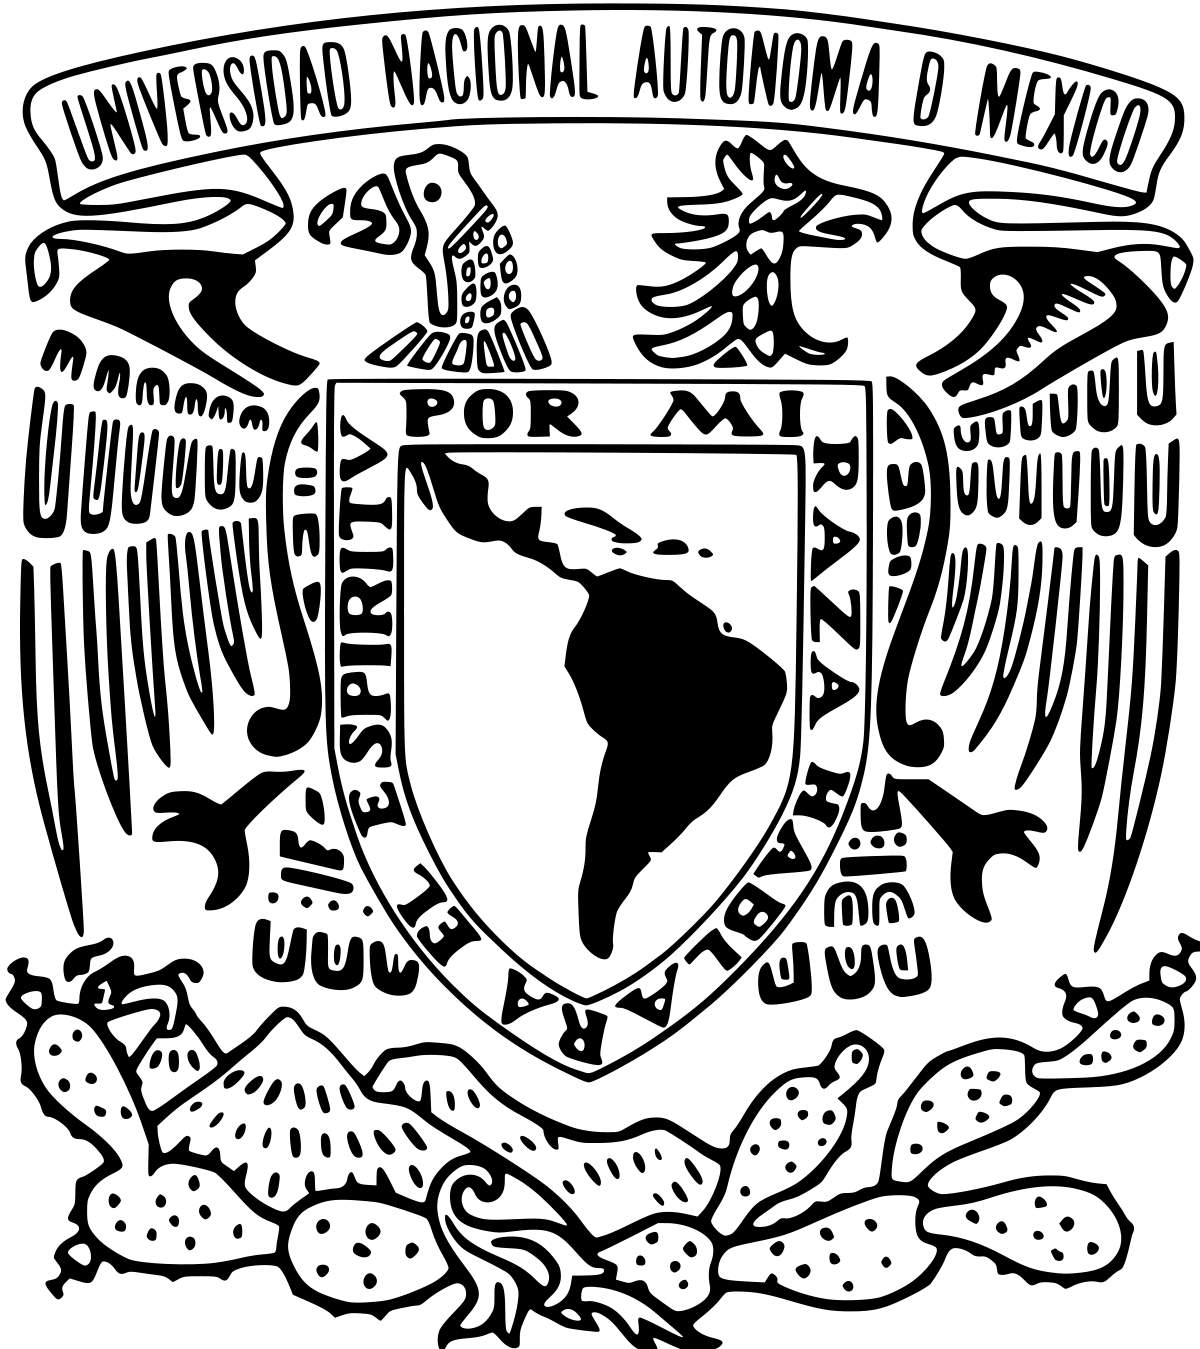
\includegraphics[height = 0.14\textheight]{recursos/Logo_UNAM.png}\par
		\end{center}
	\end{minipage}\hfill
	\begin{minipage}{10cm}

	\end{minipage}\hfill
	\begin{minipage}{3cm}
		\begin{center}
			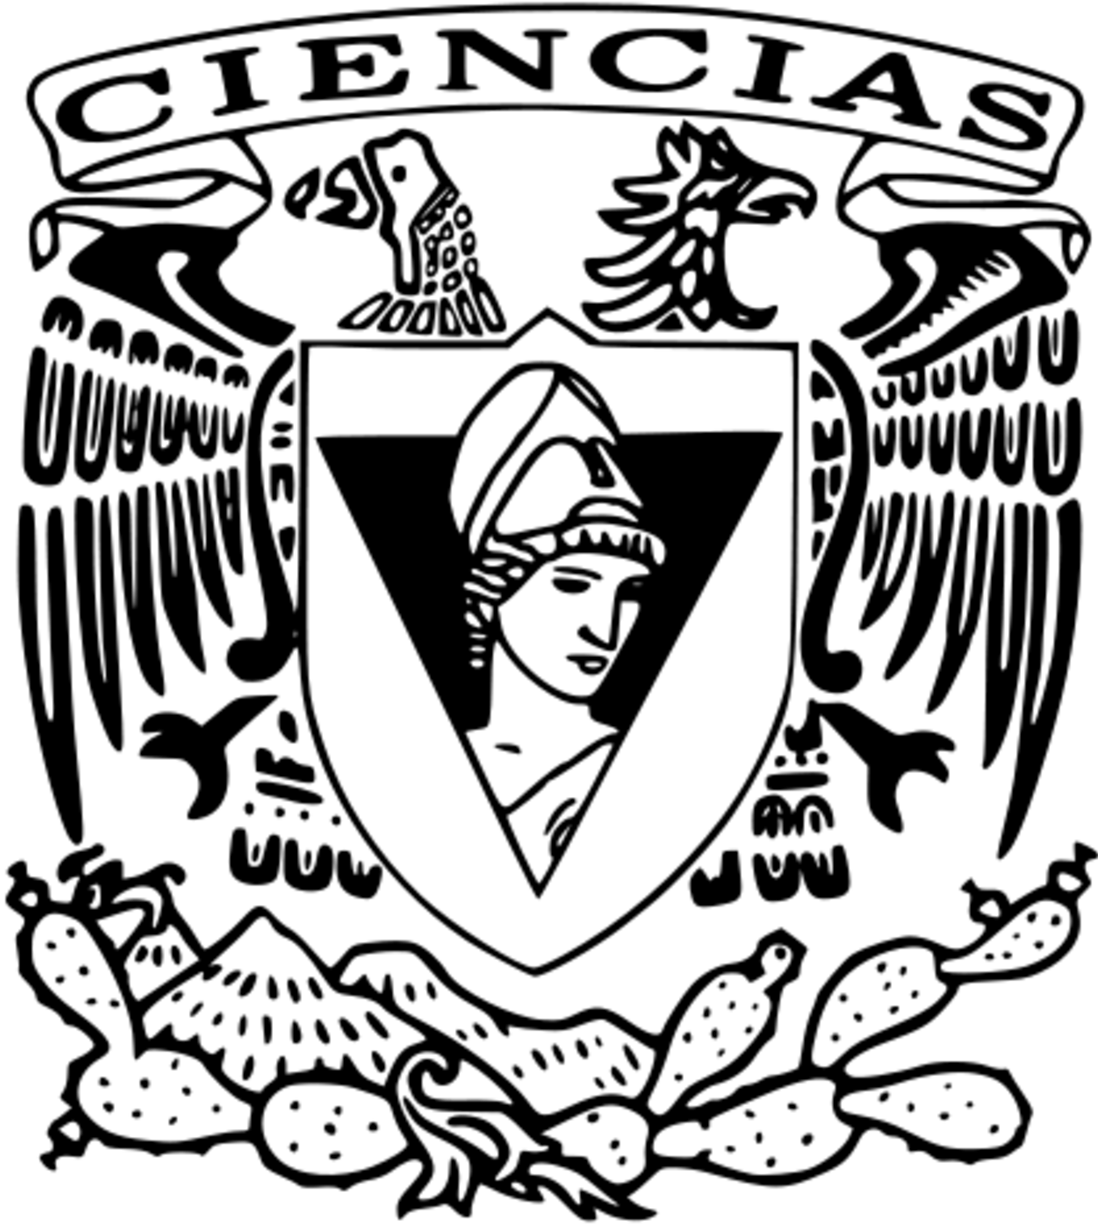
\includegraphics[height = 0.14\textheight]{recursos/Logo_FC.png}\par
		\end{center}
	\end{minipage}
	\centering
	\vspace{1cm}

	{\bfseries\LARGE Universidad Nacional Autónoma de México \par}

	\vspace{1cm}
	{\scshape\Large Facultad de Ciencias \par}
	\vspace{1cm}
	{\scshape\Large Estructuras Discretas \par}
	\vspace{1cm}
	{\scshape\Large Licenciatura en Ciencias de la Computación \par}
	\vspace{1cm}
	{\scshape\Huge Tarea 02: Lógica Proposicional.  \par}
	\vspace{3cm}
	{\itshape\Large Segundo Parcial \par}
	\vfill
	{\Large Autores: \par}
	{\Large Ramírez Mendoza Joaquín Rodrigo \par}
	{\Large Villalobos Juárez Gontran Eliut\par}
	{\Large Treviño Puebla Héctor Jerome \par}
	\vfill
	{\Large Octubre 2024 \par}
\end{titlepage}
% ---Fin de la portada de la portada
\maketitle

% Introducir aquí sus capítulos
% ------∨∨∨∨∨∨∨∨∨∨∨∨∨∨∨--------
\noindent\textbf{1. De las siguientes expresiones, identificar las proposiciones atomicas y los conectores lógicos. Traducir de lenguaje natural a lenguaje lógico:}

\begin{multicols}{2}
	\begin{enumerate}[label=\alph*)]
		\item Penélope es griega.
		\item Alonso Quijano no está cuerdo.
		\item Si Juan fue al cine, seguro que Lupe también.
		\item Melibea no está triste, porque cursó Estructuras Discretas.
		\item Juan come y bebe.
		\item Cuando María estudia, no reprueba los exámenes.
		\item Armin no fuma ni bebe.
		\item Juana juega fútbol, pero no baloncesto.
	\end{enumerate}
\end{multicols}

\textbf{a)}$p$ = \newpage
\chapter*{Ejercicio 2}
% \section*{Ejercicio 2}

Para las siguientes parejas, escribir en lenguaje natural las fórmulas:

\[
p \land q, \quad p \lor q,\quad \neg p \land q, \quad p \land \neg q, \quad \neg p \lor q, \quad p \lor \neg q
\]

\subsection*{a) $p = 1 \text{ es primo}, \quad q = 1 \text{ es natural}$}

\begin{itemize}
    \item $p \land q$: 1 es primo y 1 es natural.
    \item $p \lor q$: 1 es primo o 1 es natural.
    \item $\neg p \land q$: No es cierto que 1 sea primo y 1 es natural.
    \item $p \land \neg q$: 1 es primo y no es cierto que 1 sea natural.
    \item $\neg p \lor q$: No es cierto que 1 sea primo o 1 es natural.
    \item $p \lor \neg q$: 1 es primo o no es cierto que 1 sea natural.
\end{itemize}

\subsection*{b) $p = \text{El gato no es un vegetal}, \quad q = \text{El perro es mamífero}$}

\begin{itemize}
    \item $p \land q$: El gato no es un vegetal y el perro es mamífero.
    \item $p \lor q$: El gato no es un vegetal o el perro es mamífero.
    \item $\neg p \land q$: El gato es un vegetal y el perro es un mamifero.
    \item $p \land \neg q$: El gato no es un vegetal y el perro no es mamífero.
    \item $\neg p \lor q$: El gato es un vegetal o el perro es mamífero.
    \item $p \lor \neg q$: El gato no es un vegetal o el perro no es mamífero.
\end{itemize}

\subsection*{c) $p = 5 < 7, \quad q = 3 \leq 10$}

\begin{itemize}
    \item $p \land q$: 5 es menor que 1 y 5 es menor que 10.
    \item $p \lor q$: 5 es menor que 1 o 5 es menor que 10.
    \item $\neg p \land q$: 5 no es menor que 1 y 5 es meno que 10.
    \item $p \land \neg q$: 5 es menor que 1 y 5 no es menor que 10.
    \item $\neg p \lor q$:  5 no es menor qe 1 o 5 es mayor que 10.
    \item $p \lor \neg q$: 5 es menor que 1 o 5 no es menor que 10.
\end{itemize}

 \newpage
\chapter*{Ejercicio 3}
\section*{Ejercicio 3}

A partir de la siguiente gramática para expresiones proposicionales:

\[
E \to T \mid \neg E \mid E \land E \mid E \lor E \mid E \to E \mid (E)
\]
\[
T \to p \mid q \mid r \mid a \mid b \mid c \mid d
\]

\subsection*{a) $p \to q$}

\vspace*{\fill}
\begin{center}
\[
\begin{array}{c}
     \rightarrow \\
    / \ \backslash \\
   p   \quad  q 
\end{array}
\]
\end{center}
\vspace*{\fill}

\subsection*{b) $\neg(p \lor q)$}

\vspace*{\fill}
\begin{center}
\[
\begin{array}{c}
      \neg \\
      | \\
      \lor \\
     / \ \backslash \\
    p   \quad  q 
\end{array}
\]
\end{center}
\vspace*{\fill}

\subsection*{c) $(a \land b) \lor c \to (a \land d)$}

\vspace*{\fill}
\begin{center}
\[
\begin{array}{c}
      \rightarrow \\
      / \quad\ \quad \backslash \\
      \lor   \quad \quad \quad \land  \\
    / \ \backslash \quad\quad \quad / \ \backslash \\
   \land   \quad c \quad \quad   a \quad b\\
  / \ \backslash \quad \quad \quad \quad  \quad\\
 a   \quad  b  \quad \quad \quad\quad \quad
\end{array}
\]
\end{center}
\vspace*{\fill}

\subsection*{d) $(p \to a) \to (a \lor \neg b)$}

\vspace*{\fill}
\begin{center}
\[
\begin{array}{c}
       \rightarrow \\
      / \quad \ \backslash \\
     \rightarrow   \quad  \lor \\
    / \ \backslash \quad / \ \backslash\\
   p   \quad  a   \quad a \quad \neg\\
               \quad   | \\
                \quad   b
\end{array}
\]
\end{center}
\vspace*{\fill}

\subsection*{e) $\neg p \land \neg q \lor r$}

\vspace*{\fill}
\begin{center}
\[
\begin{array}{c}
      \lor \\
     / \ \backslash \\
    \land   \quad  r \\
   /  \ \backslash \quad \\
  \neg  \quad  \neg \quad \\
  | \quad \quad| \quad\\
  p \quad  \quad q \quad
\end{array}
\]
\end{center}
\vspace*{\fill}

\subsection*{f) $\neg a \to (b \land \neg c) \leftrightarrow \neg d$}

\vspace*{\fill}
\begin{center}
\[
\begin{array}{c}
      \leftrightarrow \\
     / \quad \ \backslash \\
    \to   \quad\quad  \neg \quad \\
   / \quad\ \backslash \quad \quad | \quad\\
   \neg    \quad \quad \land \quad d \quad \quad\\
      |\quad \quad       / \ \backslash \quad \quad \quad\\
      a\quad  \quad    b   \quad \neg  \quad \quad \\
      | \quad\\
      c \quad
\end{array}
\]
\end{center}
\vspace*{\fill}

\vspace*{\fill}\newpage
\chapter*{Ejercicio 4}
\section*{Ejercicio 4}

\textbf{4.-} Utilizar el algoritmo de analisis de proposiciones sobre las siguientes fórmulas. Dibuja los arboles binarios resultantes. Señalar si el algoritmo acepta o no la fórmula: \newline 
\begin{center}
\begin{enumerate}
\renewcommand{\theenumi}{\alph{enumi}} %Letras minúsculas 
    \item $(p \land q)\lor r) \rightarrow ( p \land s)$
    \item $(p \rightarrow q) \neg \land r$
    \item $ \neg (p \rightarrow q) \rightarrow (q \lor \neg r)$
    \item $\neg p \land \neg q \lor r$
    \item $(\neg a \rightarrow (b \land \neg c)) \leftrightarrow \neg d $
\end{enumerate}
\end{center}

%Primero recordemos el algoritmo ANALYSIS(E): (Pseudocódigo)\\
%\newline

\textbf{Para a)}
\[
((p \land q)\lor r) \rightarrow ( p \land s)
\]  \newline
El algoritmo si acepta la fórmula y genera el siguiente árbol binario: \newline

\begin{center}
\[
\begin{array}{c}
\rightarrow \\
/ \quad \ \backslash \\
\lor \quad  \quad  \land \\
/ \ \backslash \quad / \ \backslash \\
\land \quad r \quad p \quad s \\
/ \ \backslash \quad \quad \quad \quad \quad\\
p \quad q \quad \quad \quad \quad \quad  \\
\end{array}
\]
\end{center}\\


\textbf{Para b)}
\[
(p \rightarrow q) \neg \land r
\]  \newline
El algoritmo NO acepta la fórmula y  NO genera el
árbol binario esto por no ser $wff$ (well formed formula).\\
\newline
El algoritmo regresa fail, puesto que al evaluar rankL(E) lo que recibe es: \\
$ (p \rightarrow q) \neg$ lo cual es ínvalido puesto que al tener la negación el algoritmo requiere el caso de tipo $\neg (E)$ lo cual no se tiene en este caso.\\
Regresa $Fail$.\\
\newline

\textbf{Para c)}
\[
\neg (p \rightarrow q) \rightarrow (q \lor \neg r)
\]  \newline
El algoritmo si acepta la fórmula y genera el siguiente árbol binario: \newline

\begin{center}
\[
\begin{array}{c}
\rightarrow \\
/ \quad \backslash \\
\neg \quad \quad \lor \\
\quad | \quad \quad / \quad \backslash \\
\quad \rightarrow \quad  q \quad \neg \\
/ \quad \backslash \quad \quad \quad | \\
p \quad \quad q \quad \quad \quad r\\
\end{array}
\]
\end{center}

\textbf{Para d)}
\[
\neg p \land \neg q \lor r
\]  \newline
El algoritmo si acepta la fórmula y genera el siguiente árbol binario: \newline

\begin{center}
\[
\begin{array}{c}
\land \\
/ \quad \backslash \\
\neg \quad \quad \lor \\
\quad | \quad \quad / \quad \backslash \\
\quad p \quad \quad  \neg \quad r \\
\quad \quad \quad | \quad \\
\quad \quad \quad q \quad \\
\end{array}
\]
\end{center}

\textbf{Para e)}
\[
(\neg a \rightarrow (b \land \neg c)) \leftrightarrow \neg d
\]  \newline
El algoritmo si acepta la fórmula y genera el siguiente árbol binario: \newline

\begin{center}
\[
\begin{array}{c}
\leftrightarrow \\
/ \quad \backslash \\
\rightarrow \quad \quad \neg \\
/ \quad \backslash \quad \quad | \\
\neg \quad \land \quad \quad d \\
| \quad / \quad \backslash \quad \quad  \\
a \quad b \quad \neg \quad \quad \\
\quad | \\
\quad c \\
\end{array}
\]
\end{center}\newpage
\chapter*{Ejercicio 5}
% \section*{Ejercicio 5}

\textbf{5.-} Demostrar que el algoritmo de analisis ANALYSIS(E) de expresiones proposicionales es completo, cuando la expresion tiene longitud finita. \\
\newline
\begin{center}
    Demostracion sobre los pasos del algoritmo
\end{center}

Despúes de haver visto el pseudocódigo del algoritmo, veremos el algoritmo en casos: \\
\begin{align*}
ANALYSIS(E) = \begin{cases}
    Tree (void,E,void)  & \text{si } E=\text{prop. atómica}. \\
    Tree (void,\neg, ANALISIS(E) & \text{si } E=\neg E \\
    Tree (ANALYSIS(rankL(E)),\diamondsuit,ANALYSIS(rankR(E)) & \text{si } E=E \diamondsuit E \\
\end{cases}
\end{align*}
\newline
\textbf{1) CASO BASE:}\\
\newline
Para E = prop. atómica (var p,q... o constante $\bot$ o $\top$)
Regresa $tree (void,E,void)$, si se cumple el algoritmo el regresa el árbol de E. \\
\newline

\textbf{2) HIPOTESIS DE INDUCCIÓN:}\\
\newline
Sean A y B proposiciones con las longitudes de A y B menores que $n$\\
\begin{itemize}
    \item ANALYSIS($A$) regresa el árbol sintáctico de A (se cumple para A).
    \item ANALYSIS($B$) regresa el árbol sintáctico de B (se cumple para B).
    %\item ANALYSIS($\neg A$) regresa el árbol sintáctico de $\neg A$ (se cumple para la negación).
    %\item ANALYSIS($A \diamondsuit B$) regresa el árbol sintáctico de $A \diamondsuit B$ (se cumple para operadores binarios).
\end{itemize}

\textbf{3) PASO INDUCTIVO:}\\
\newline
Por Demostrar para: ANALYSIS(E) es completo cuando E es de longitud $n$. \\
Tenemos dos casos, el caso de la negación y el caso con un operador binario:\\
\begin{itemize}
    \item Si $E=\neg A$, en esta situación caemos en el segundo caso de nuestro algoritmo\\
    Por lo tanto se debe aplicar $\neg ANALYSIS(A)$, y por \textbf{H.I.} sabemos que $ANALYSIS(A)$ se cumple. Así podemos decir que el algoritmo se cumple también para este caso.
    \item Si $E = A \diamondsuit B$, en esta situación se presenta el tercer caso definido por nuestro algoritmo\\
    Por lo tanto como se generará, \\ $Tree(ANALYSIS(rankL(E)),\diamondsuit,Tree(ANALYSIS(rankR(E)))$, por la función MainOP sabemos que $rankL(E)=A$ y $rankR(E)=B$, así tenemos $Tree(ANALYSIS(A),\diamondsuit,Tree(ANALYSIS(B))$, por \textbf{H.I.} sabemos que $ANALYSIS(A)$ y $ANALYSIS(B)$ se cumplen. Así podemos decir que el algoritmo también se cumple para este caso.
\end{itemize}
Asi vemos como se funciona para E cuando E es compuesta de longitud $n$. \\
\newline 
Además se E es $wff$ siempre llegaremos a una E atómica y si E NO es $wff$ el algoritmo regresará $fail$. \\
\newline
\textbf{Por lo tanto}, Demostramos que el algoritmo de ANALYSIS(E) es completo cuando la expresión tiene longitud finita.\newpage
\chapter*{Ejercicio 6}
% \section*{Ejercicio 6}

Elaborar las tablas de verdad para las siguientes propocisoiones:
\[
a) \quad \neg (p \land q), \quad b)\quad \neg (p \lor q),\quad c) \quad (r \lor ( p \land q)) \to r,\] 
\[\quad d) \quad (p \land ( r \land q) ) \to  q, \quad e) \quad (p \to q) \leftrightarrow ( p \to r)
\] \\

\textit{a) }
% Tabla (a)
\[
\begin{array}{|c|c|c|c|c|}
\hline
p & q & p \land q & \neg (p \land q) \\
\hline
\text{V} & \text{V} & \text{V} & \text{F} \\
\hline
\text{V} & \text{F} & \text{F} & \text{V} \\
\hline
\text{F} & \text{V} & \text{F} & \text{V} \\
\hline
\text{F} & \text{F} & \text{V} & \text{V} \\
\hline
\end{array}
\]  


\textit{b) }
% Tabla (b)
\[
\begin{array}{|c|c|c|c|}
\hline
p & q & p \lor q & \neg (p \lor q) \\
\hline
\text{V} & \text{V} & \text{V} & \text{F} \\
\hline
\text{V} & \text{F} & \text{F} & \text{F} \\
\hline
\text{F} & \text{V} & \text{F} & \text{F} \\
\hline
\text{F} & \text{F} & \text{F} & \text{V} \\
\hline
\end{array}
\]

\textit{c) }
% Tabla (c)
\[
\begin{array}{|c|c|c|c|c|}
\hline
p & q & r & r \lor (p \land q) & (r \lor (p \land q)) \rightarrow r \\
\hline
\text{V} & \text{V} & \text{V} & \text{V} & \text{V} \\
\hline
\text{V} & \text{V} & \text{F} & \text{V} & \text{F} \\
\hline
\text{V} & \text{F} & \text{V} & \text{V} & \text{V} \\
\hline
\text{V} & \text{F} & \text{F} & \text{F} & \text{V} \\
\hline
\text{F} & \text{V} & \text{V} & \text{V} & \text{V} \\
\hline
\text{F} & \text{V} & \text{F} & \text{F} & \text{V} \\
\hline
\text{F} & \text{F} & \text{V} & \text{V} & \text{V} \\
\hline
\text{F} & \text{F} & \text{F} & \text{F} & \text{V} \\
\hline
\end{array}
\]

\textit{d) }

%Tabla(d)
\[
\begin{array}{|c|c|c|c|c|c|c|}
\hline
p & q & r & r  \land q & p \land (r \land q) & (p \land (r \land q )) \to q\\
\hline
\text{V} & \text{V} & \text{V} & \text{V}&\text{V} & \text{V} \\
\hline
\text{V} & \text{V} & \text{F} & \text{F} & \text{F} & \text{V}\\
\hline
\text{V} & \text{F} & \text{V} & \text{F} & \text{F} & \text{V} \\
\hline
\text{V} & \text{F} & \text{F} & \text{F} & \text{F} & \text{V}\\
\hline
\text{F} & \text{V} & \text{V} & \text{V} & \text{F} & \text{V}\\
\hline
\text{F} & \text{V} & \text{F} & \text{F} & \text{F} & \text{V}\\
\hline
\text{F} & \text{F} & \text{V} & \text{F} & \text{F} & \text{V}\\
\hline
\text{F} & \text{F} & \text{F} & \text{F} & \text{F} & \text{V}\\
\hline
\end{array}
\]

\textit{e) }
%Tabla (e)
\[
\begin{array}{|c|c|c|c|c|c|}
\hline
p & q & r & p \rightarrow q & p \rightarrow r & (p \rightarrow q) \leftrightarrow (p \rightarrow r) \\
\hline
\text{V} & \text{V} & \text{V} & \text{V} & \text{V} & \text{V} \\
\hline
\text{V} & \text{V} & \text{F} & \text{V} & \text{F} & \text{F} \\
\hline
\text{V} & \text{F} & \text{V} & \text{F} & \text{V} & \text{F} \\
\hline
\text{V} & \text{F} & \text{F} & \text{F} & \text{F} & \text{V} \\
\hline
\text{F} & \text{V} & \text{V} & \text{V} & \text{V} & \text{V} \\
\hline
\text{F} & \text{V} & \text{F} & \text{V} & \text{V} & \text{V} \\
\hline
\text{F} & \text{F} & \text{V} & \text{V} & \text{V} & \text{V} \\
\hline
\text{F} & \text{F} & \text{F} & \text{V} & \text{V} & \text{V} \\
\hline
\end{array}
\]\newpage
\chapter*{Ejercicio 7}
\textbf{7. Demuestra que la función del complemento regresa la negación de la fórmula.}

Esto es, que $comp(E)=\neg E$\\
\textbf{Proposición.} Sea $comp$ la siguiente función recursiva:
% \begin{alignat*}{2}
% 	comp(\top)      & = \bot                  & \quad & (i)   \\
% 	comp(\bot)      & = \top                  & \quad & (ii)  \\
% 	comp(p)         & = \neg p                & \quad & (iii) \\
% 	comp(\neg Q)    & = \neg comp(Q)          & \quad & (iv)  \\
% 	comp(P \land Q) & = comp(P) \land comp(Q) & \quad & (v)   \\
% 	comp(P \lor Q)  & = comp(P)\lor comp(Q)   & \quad & (vi)  \\
% \end{alignat*}
\begin{enumerate}
	\item $comp(\top) = \bot,\;comp(\bot) = \top,\;comp(p) = \neg p$ son atómicas.
	\item Si P y Q son fórmulas: $comp(\neg Q) = \neg comp(Q),\;comp(P \land Q) = comp(P) \land comp(Q),\;comp(P \lor Q) = comp(P)\lor comp(Q)$
\end{enumerate}
\indent Entonces se cumple que $comp(E)=\neg E$
\noindent\\
\textbf{Demostración:} Por inducción estructural sobre las fórmulas.\\
\indent
\textbf{Caos base.} Cuando $E$ es atómica tal que $E=p$ donde $p$ es una proposición ó $E=\top$ ó $E=\bot$
\begin{multicols}{3}
	\begin{alignat*}{2}
		E       & = p \text{ tal que } & \quad & \text{p es atómica}  \\
		comp(E) & = comp(p)                                           \\
		        & = \neg p             & \quad & \text{Por p atómica} \\
	\end{alignat*}

	\begin{alignat*}{2}
		E=\top\therefore                         \\
		comp(E) & = comp(\top)                   \\
		        & = \neg \top  & \quad & \text{} \\
		        & = \bot       & \quad & \text{} \\
	\end{alignat*}

	\begin{alignat*}{2}
		E=\bot\therefore                         \\
		comp(E) & = comp(\bot)                   \\
		        & =\neg \bot   & \quad & \text{} \\
		        & =\top        & \quad & \text{} \\
	\end{alignat*}
\end{multicols}

\textbf{Hipótesis de inducción:} Supongamos que se cumple para dos proposiciones $P$, $Q$ tales que  $comp(P)=\neg P$ y $comp(Q)=\neg Q$\\
\textbf{Paso inductivo: Por demostrar que se cumple para los pasos recurisvos 
de la función $comp(E)=\neg E$}
\begin{multicols}{3}
	\noindent
	\begin{align*}
		comp(\neg Q)              & = \neg comp(Q) \\
		\text{Por H.I}            & = \neg \neg Q  \\
		\text{Por doble negación} & =  Q           \\
	\end{align*}
\noindent
	\begin{align*}
		comp(P\land Q)      & = comp(P)\land comp(Q) \\
		\text{Por H.I}      & = \neg P \land \neg Q  \\
		\text{Por deMorgan} & = \neg (P\lor Q)       \\
	\end{align*}
\noindent
	\begin{align*}
		comp(P\lor Q)       & = \neg comp(P) \lor \neg comp(Q) \\
		\text{Por H.I}      & = \neg P \lor \neg Q             \\
		\text{Por deMorgan} & = \neg (P\land Q)                \\
	\end{align*}
\end{multicols}

$\therefore$ Se concluye que se cumple para todos los casos recurisvos de la función del complemento se cumple que$$comp(E)=\neg E\text{, para cualquier fórmula}$$\newpage
\textbf{8. Demostra que a partir de los conjuntos de proposiciones dados $\Gamma$, si las siguientes proposiciones son o no consecuencias lógicas utilizando interpretaciones.}
\begin{multicols}{2}
	\begin{enumerate}[label=\alph*)]
		\item $\Gamma = \{p\land q, r\lor q\}$, proposición: $p \land q\lor r$
		\item $\Gamma = \{p\leftrightarrow q,p\rightarrow \neg r,r\rightarrow s\}$, proposición: $q\rightarrow s$
		\item $\Gamma = \{p\leftrightarrow q,p\rightarrow \neg r,r\rightarrow s\}$, proposición: $\neg (p\land r)$
		\item $\Gamma = \{p\lor q, q\rightarrow r, \neg r \lor s\}$, proposición: $(p\lor q)\rightarrow s$
		\item $\Gamma = \{p\land q, q\rightarrow r, r \lor \neg s\}$, proposición: $(p \land q)\rightarrow r$
	\end{enumerate}
\end{multicols}

\textbf{Mostrar que a) 	$\Gamma=\{p\land q, r\lor q\} \vDash p \land q\lor r$.}\\
Suponemos la veracidad de $\mathcal{I}(\Gamma)=1$\\
Sea $\mathcal{I}$ un modelo $\Gamma$. Tenemos que demostrar que $\mathcal{I}((p \land q)\lor r)=1$.\\
Como $\mathcal{I}(p\lor q)=1$, entonces $\mathcal{I}(p)=1=\mathcal{I}(q)$ y para $\mathcal{I}(r\lor q)$ tenemos dos casos\\
\indent i) Cuando $\mathcal{I}(r)=1$, y como $\mathcal{I}(q)=1$ entonces $\mathcal{I}(q\lor r)=1$ siempre, por lo que $\mathcal{I}(p \land q\lor r)=1$ dodo que $\mathcal{I}(p \land q)=1$ y $\mathcal{I}(r)=1$\\
\indent ii) Por otro lado, Cuando $\mathcal{I}(r)=0$, como $\mathcal{I}(q)=1$, entonces $\mathcal{I}(q\lor r)=1$\\
$\therefore \mathcal{I}((p\land q)\lor r)=1$\\
\indent
$\therefore$ se concluye que es onsecuencia lógica. $\blacksquare$
\vspace{10px}

\textbf{Mostrar que b)} $\Gamma = \{p\leftrightarrow q,p\rightarrow \neg r,r\rightarrow s\} \vDash q\rightarrow s$\\
Suponemos la veracidad de $\mathcal{I}(\Gamma)=1$\\
Tenemos dos casos:\\
 \indent i) Si $\mathcal{I}(q)=0$ entonces $\mathcal{I}(q\rightarrow s)=1$ por lo que es trivial.\\
\indent ii) Si $\mathcal{I}(q)=1$, entonces $\mathcal{I}(p)=1$ para que sea $\mathcal{I}(p\leftrightarrow q)=1$, por lo que $\mathcal{I}(\neg r)=1$ necesariamente, pues $\mathcal{I}(p\rightarrow \neg r)=1$, entonces $\mathcal{I}(r)=0$, quiere decir que $\mathcal{I}(r\rightarrow s)=1$, en particular para $\mathcal{I}(s)=0$, por lo que, si $\mathcal{I}(q)=1$, como lo definimos anteriormente y si $\mathcal{I}(s)=0$, quiere decir que $\mathcal{I}(r\rightarrow s)=0$\\
$\therefore$ No es consecuencia lógica $\blacksquare$
\vspace{10px}

\textbf{Mostrar que c) $\Gamma = \{p\leftrightarrow q,p\rightarrow \neg r,r\rightarrow s\} \vDash \neg (p\land r)$}\\
Suponemos la veracidad de $\mathcal{I}(\Gamma)=1$\\
Tenemos dos casos:\\
\indent i) Si $\mathcal{I}(p)=0$, entonces $\mathcal{I}(\neg(p\land r))=1$ pues $\mathcal{I}(p\land r)=0$.\\
\indent ii) Si $\mathcal{I}(p)=1$ como $\mathcal{I}(p \leftrightarrow q)=1$ entonces $\mathcal{I}(q)=1$, esto quiere decir que, como $\mathcal{I}(q\rightarrow \neg r)=1$, tiene que pasar que $\mathcal{I}(\neg r)=1$, por lo que $\mathcal{I}(r)=0$.\\
Esto quiere decir que $\mathcal{I}(p\land r)=0$ y $\mathcal{I}(\neg (p\land r))=1$\\
$\therefore$ Si es consecuencia lógica.$\blacksquare$
\vspace{10px}

\textbf{Mostrar que d) $\Gamma = \{p\lor q, q\rightarrow r, \neg r \lor s\}\vDash(p\lor q)\rightarrow s$}\\
Suponemos la veracidad de $\mathcal{I}(\Gamma)=1$\\
Tenemos dos casos:\\
\indent i)Supongamos que $\mathcal{I}(q)=1$, dado que $\mathcal{I}(p\rightarrow r)=1$ quiere decir que $\mathcal{I}(r)=1$, entonces $\mathcal{I}(\neg r)=0$, y como $\mathcal{I}(\neg r\lor s)=1$ tiene que pasar que $\mathcal{I}(s)=1$, dado que suponemos que $\mathcal{I}(p\lor q)=1$ es necesario que $\mathcal{I}(p)=1$ pues $\mathcal{I}(q)=0$ como suposimos anteriormente. $\therefore\mathcal{I}((p\lor q)\rightarrow s)=1$\\
\indent ii)Supongamos$\mathcal{I}(q)=0$, entonces, en particular, suponemos que $\mathcal{I}(r)=0$, esto significa que $\mathcal{I}(\neg r)=1$, como $\mathcal{I}(\neg r \lor s)=1$ puede pasar que $\mathcal{I}(s)=0$, y dado que $\mathcal{I}(p\lor q)=1$ tiene que pasar que $\mathcal{I}(p)=1$ entonces decimos que $\mathcal{I}((p\lor q)\rightarrow s)=0$ puesto que $\mathcal{I}(p\lor q)=1$ pero $\mathcal{I}(s)=0$\\
$\therefore$ No es consecuencia lógica. $\blacksquare$
\vspace{10px}

\textbf{Mostrar que e) $\Gamma = \{p\land q, q\rightarrow r, r \lor \neg s\}\vDash (p \land q)\rightarrow r$}\\
Suponemos la veracidad de $\mathcal{I}(\Gamma)=1$\\
Dado que $\mathcal{I}(p\land q)=1$ tiene que pasar que $\mathcal{I}(p)=1=\mathcal{I}(q)$, entonces es necesario que $\mathcal{I}(r)=1$ pues $\mathcal{I}(q\rightarrow r)=1$, quiere decir se cumple 
$\mathcal{I}(r \lor \neg s)=1$ pues basta que al menos uno sea $1$ para que la proposición se cumpla, lo que quiere decir que $\mathcal{I}((p\land q)\rightarrow r)=1$\\
$\therefore$ Es consecuencia lógica. $\blacksquare$\newpage
\chapter*{Ejercicio 10}
% \section*{Ejercicio 10}

\textbf{10.} Probar que el operador de disyuncion exclusiva (XOR) $p \veebar q$ es equivalente a $\neg (p \land q) \land (p \lor q)$.\\
\newline
(Proposiciones equivalentes). Decimos que dos formulas proposicionales $p$ y $q$ son equivalentes si y solo si en todos sus posibles estados tienen el mismo valor de verdad.
Por lo tanto para probar la equivalencia de $p \veebar q$ y $\neg (p \land q) \land (p \lor q)$ generaremos su tabla de verdad. \\
\newline
\[
\begin{array}{|c|c|c|c|c|c|c|}
\hline
p & q & p \land q & p \lor q & \neg (p \land a) & \neg (p \land q) \land (p \lor q) & p \veebar q \\
\hline
0 & 0 & 0 & 0 & 1 & 0 & 0 \\
\hline
0 & 1 & 0 & 1 & 1 & 1 & 1 \\
\hline
1 & 0 & 0 & 1 & 1 & 1 & 1 \\
\hline
1 & 1 & 1 & 1 & 0 & 0 & 0 \\
\hline
\end{array}
\]

Dado este resultado podemos ver que los valores de $\neg (p \land q) \land (p \lor q)$ y $p \veebar q$ son iguales en todos sus posibles estados. Por lo tanto son proposiciones equivalentes.
\newpage
\chapter*{Ejercicio 11}
\section*{Ejercicio 11}

Demostrar que dada una fórmula de lógica proposicional $E$, la altura es menor o igual que la longitud. Esto es $h(E) \leq \text{len}(E)$. \\

\begin{enumerate}
    \item[1)] Caso base: consideramos que $\text{len}(E) = 1$ y altura $h(E) = 1$, entonces este caso hace que se cumpla que
    \[
    h(E) \leq \text{len}(E)
    \]
    por lo tanto, es correcto.

    \item[2)] Hipótesis de inducción: suponemos que para $E_1$ y $E_2$ se cumple que
    \[
    h(E_1) \leq \text{len}(E_1) \quad \text{y} \quad h(E_2) \leq \text{len}(E_2).
    \]
    Queremos probar que para las fórmulas $E = E_1  \diamondsuit E_2$, o $\neg E_1$, también se cumple la desigualdad.

    \begin{itemize}
        \item Caso $E = E_1 \diamondsuit E_2$:
        \begin{itemize}
            \item[]  Longitud:
            \[
            \text{len}(E_1 \diamondsuit E_2) = \text{len}(E_1) + \text{len}(E_2) + 1
            \]
            \item[] Altura:
            \[
            h(E_1 \diamondsuit E_2) = 1 + \max(h(E_1), h(E_2))
            \]
            Por la hipótesis de inducción, tenemos que $h(E_1) \leq \text{len}(E_1)$ y $h(E_2) \leq \text{len}(E_2)$. Entonces:
            \[
            h(E_1 \land E_2) = 1 + \max(h(E_1), h(E_2)) \leq 1 + \max(\text{len}(E_1), \text{len}(E_2)) \leq \text{len}(E_1) + \text{len}(E_2) + 1
            \]
            \[
            = \text{len}(E_1 \land E_2)
            \]
            Por lo tanto, se cumple que $h(E_1 \land E_2) \leq \text{len}(E_1 \land E_2)$.
        \end{itemize}
        \item Caso $E = \neg E_1$:
        \begin{itemize}
            \item []Longitud:
            \[
            \text{len}(\neg E_1) = \text{len}(E_1) + 1
            \]
            \item[] Altura:
            \[
            h(\neg E_1) = h(E_1) + 1
            \]
            Por la hipótesis de inducción, sabemos que $h(E_1) \leq \text{len}(E_1)$, entonces se cumple que
            \[
            h(\neg E_1) = h(E_1) + 1 \leq \text{len}(E_1) + 1 = \text{len}(\neg E_1)
            \]
            Así, se cumple que $h(\neg E_1) \leq \text{len}(\neg E_1)$.
        \end{itemize}
    \end{itemize}
\end{enumerate}

Conclusión: por inducción, sabemos que para una fórmula proposicional $E$, se cumple que
\[
h(E) \leq \text{len}(E)
\]
\end{document}